% !TEX root = cha-soa.tex
\documentclass[../../main.tex]{subfiles}

\begin{document}

\subsection{Cartographic Visualization}

Kuhn~\etal~\citebibliography{Kuhn2010a} introduced \emph{Software Cartography}, an approach that represents software systems as maps. Its main goal is to place software entities according to their semantic similarity. Entities with similar vocabulary are placed close to each other, while less similar entities are placed farther apart. This also provides a consistent layout that remains stable as the software evolves, unlike layouts based on physical structures such as package hierarchies.

To create the map, Software Cartography uses the vocabulary of the source code as a measure of similarity. Source files are represented using term-frequency histograms and processed with Latent Semantic Indexing (LSI). Multidimensional Scaling (MDS) then maps the resulting high-dimensional representation down to a two-dimensional space. In the result, semantically similar entities are placed close to each other.

The map can then be enriched with cartographic elements to represent additional software properties. For example, the height of the landscape is represented by the number of lines of code (KLOC), then hill shading and contour lines are added to render more aesthetically appealing landscapes. An example of a software map generated using this approach is shown in \figref{fig:cartography}.

\begin{figure}[h]
    \centering
    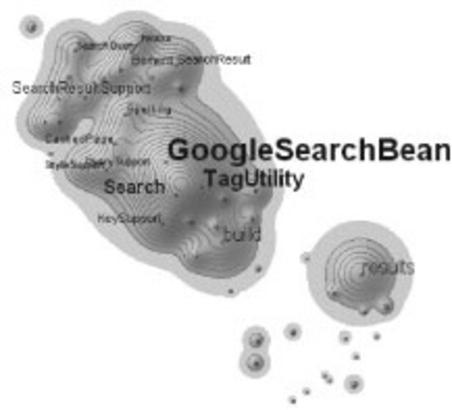
\includegraphics[width=0.45\linewidth]{figures/soa/cartography}
    \caption[Example of a Software Map]{Example of a Software Map~\citebibliography{Kuhn2010a}.}
    \label{fig:cartography}
\end{figure}


\end{document}